%!TEX root = document.tex

Hem implementat dos algorismes diferents d'obtenció de l'estat inicial per tal de poder comparar-los i veure quin porta a millors estats finals. A priori, tal com funciona la cerca local, si l'estat inicial de partença és bo hi ha més probabilitats d'obtenir un resultat òptim.  En ambdós casos, els estats es troben dins l'espai de solucions i per això els anomenem solucions inicials.

\subsubsection{Solució inicial aleatòria}

Aquesta solució (mètode anomenat \textbf{solIni2}) té com a prioritat la rapidesa i l'aleatorietat de la seva obtenció i no la seva qualitat. En cada iteració es procedeix a afegir una parada escollida a l'atzar per cada ruta. Quan totes les parades han estat assignades a alguna ruta, l'algorisme s'atura. La configuració obtinguda no només és solució del problema, sinó que compleix amb la restricció addicional proposada d'entrada. L'assignació de parades és homogènia i basada en el factor aleatori. El cost de la funció és lineal de l'ordre $\Theta(P)$.

\subsubsection{Solució inicial de qualitat}

Aquesta solució (mètode anomenat \textbf{solIni1}), en canvi, intenta ser bona d'entrada amb l'esperança que facilitarà als algoritmes de cerca local arribar a un bon òptim local o bé a l'òptim global. Per fer-ho, la solució incorpora coneixement del problema a minimitzar. 

En concret, el procediment consisteix en anar afegint a cada ruta la parada més propera a l'última parada afegida i, a la vegada, més propera a la parada final. Aquesta última restricció evita que apareguin \emph{recorreguts en cercle} (veure gràfics 1 i 2). Aquestes comprovacions faciliten que la solució obtinguda segueixi el primer criteri a optimitzar (minimitzar el recorregut de les rutes), però no garanteixen explícitament millores pel que fa al segon criteri. Tanmateix, pel fet d'escollir sempre les distàncies menors entre parades estarem també reduint la diferència de la separació entre parades (que altrament seria aleatòria), així que també oferirà millors resultats pel que fa al compliment del segon criteri a optimitzar (minimitzar diferència entre separació de parades) respecte a la solució aleatòria.

En definitiva, aquest algorisme ofereix una solució raonablement bona amb un cost de l'ordre $\Theta(K * P)$.

\graphicspath{{./images}}

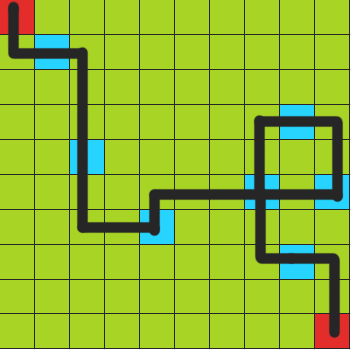
\includegraphics{grafic_sense_control_final.jpg}

Gràfic 1: No es té en compte la distància entre la parada candidata i el final, les solucions poden caure en recorreguts en cercle.

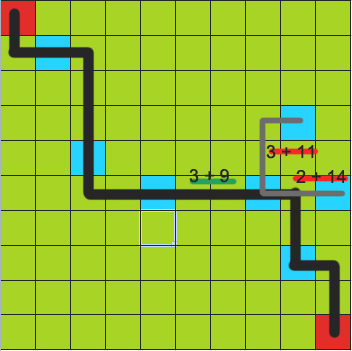
\includegraphics{grafic_amb_control_final.jpg}

Gràfic 2: Es tenen en compte ambdues distàncies, el problema desapareix.